
\documentclass[calculator,allquestions,datasheet,solutions]{exam_newMarcus2}
%\documentclass[calculator,allquestions,datasheet,Pens]{exam_newMarcus2}

% The full list of class options are
% calculator : Allows approved calculator use.
% datasheet : Adds a note that data sheet are attached to the exam.
% handbook : Allows the use of the engineering handbook.
% resit : Adds the resit markings to the paper.
% sample : Adds conspicuous SAMPLE markings to the paper
% solutions : Uses the contents of \solution commands (and \solmarks) to generate a solution file

\usepackage{pdfpages}   
\usepackage{lscape,comment}   
 
\coursecode{EX3029}%% 
\coursetitle{Chemical Thermodynamics}
 
\examtime{00.00--00.00}%
\examdate{15}{12}{2017}% 
\examformat{Attempt ALL questions. \\ Each question is worth 20 marks.}

% Other symbols
\newcommand{\frc}{\displaystyle\frac}
\newcommand{\br}[1]{\!\left( #1 \right)}
\newcommand{\abs}[1]{\left| #1 \right|}
\newcommand{\fracd}[2]{\frac{\mathrm{d} #1}{\mathrm{d} #2}}
\newcommand{\fracp}[2]{\frac{\partial #1}{\partial #2}}
\renewcommand{\d}[1]{\mathrm{d} #1 } 
\newcommand{\Ma}{\mathrm{M\!a}} 
\newcommand{\eg}{{\it e.g., }}
\newcommand{\ie}{{\it i.e., }}
\newcommand{\wrt}{{\it wrt }}
\newcommand{\Partial}[3][error]{\left(\frc{\partial #1}{\partial #2}\right)_{#3}}
\newcommand{\mfr}[3][error]{#1_{#2}^{\left(#3\right)}} 
\newcommand{\summation}[3][error]{\sum\limits_{#2}^{#3}#1}


\begin{document}


%%%
%%% Question 01 
%%%
\begin{question}
     In the design of a new process, nitrogen dioxide $\left(\text{NO}_{2}\right)$ is produced through the decomposition of nitrogen tetroxide $\left(\text{N}_{2}\text{O}_{4}\right)$,
        \begin{displaymath}
           N_{2}O_{4} (g) \Longleftrightarrow 2 NO_{2} (g),
        \end{displaymath}
        with Gibbs energy of formation at 25$^{\circ}$C,
        \begin{displaymath}
           \left(\Delta G^{\circ}_{\text{f,298}}\right)_{N_{2}O_{4}} = 97.89 \text{ kJ.mol}^{-1} \text{ and } \left(\Delta G^{\circ}_{\text{f,298}}\right)_{NO_{2}} = 51.31 \text{ kJ.mol}^{-1},
        \end{displaymath}
        and the standard enthalpy of reaction at 25$^{\circ}$C is 56.189 kJ.mol$^{-1}$. For such decomposition, three scenarios are investigated to overall conversion:
        \begin{enumerate}[A.]
           \item Decomposition at 25$^{\circ}$C;
           \item Initial dilution with inert N$_{2}$ prior to the decomposition at 25$^{\circ}$C;
           \item Decomposition at 126.85$^{\circ}$C.
        \end{enumerate}
        Calculate the composition of the species in equilibrium for:
     \begin{enumerate}[a)]
        \item Scenario A;~\marks{5}
%%%%%%%%%%%%%%%%%%%%%%%%%%%%%%%%%%%%%%%%%%%%%%%%%%%%%%%%%%%%%%%%%%       
           \solution{The equilibrium constant is
         \begin{displaymath}
             K = \exp\left(-\frc{\Delta G^{\circ}_{r,298}}{RT}\right) = \frc{a_{NO_{2}}^{2}}{a_{N_{2}O_{4}}} = \frc{\left(\frc{y_{NO_{2}}P}{P^{\circ}_{NO_{2}}}\right)^{2}}{\left(\frc{y_{N_{2}O_{4}}P}{P^{\circ}_{N_{2}O_{4}}}\right)} = \frac{\left(y_{NO_{2}}\right)^{2}}{\left(y_{N_{2}O_{4}}\right)},
         \end{displaymath}
         where the standard Gibbs energy of reaction is~\solmarks{1/5}
         \begin{eqnarray}
           \Delta G^{\circ}_{r,298} &=& \sum\limits_{i}\nu_{i}\Delta G^{\circ}_{\text{f,298}} \nonumber \\
                             &=& (+2).\left(\Delta G^{\circ}_{\text{f,298}}\right)_{NO_{2}} + (-1).\left(\Delta G^{\circ}_{\text{f,298}}\right)_{N_{2}O_{4}} \nonumber \\ 
                             &=& 4730 \text{ J/mol}, \nonumber
         \end{eqnarray}
         and the equilibrium constant,
         \begin{displaymath}
             K = \exp\left(-\frc{\Delta G^{\circ}_{r,298}}{RT}\right) = 0.1484 = \frac{\left(y_{NO_{2}}\right)^{2}}{\left(y_{N_{2}O_{4}}\right)}
         \end{displaymath}
         Composition and reaction coordinate are related through
         \begin{displaymath}
            y_{i} = \frc{n_{i,0} + \nu_{i}\varepsilon}{n_{0}+\nu\epsilon},
         \end{displaymath}
         where, assuming that the initial number of moles are $n_{N_{2}O_{4},0}=1$ and $n_{NO_{2},0}=0$, an $\nu= 2-1 = 1$,~\solmarks{1/5}
         \begin{displaymath}
            y_{N_{2}O_{4}} = \frc{1-\varepsilon}{1+\varepsilon}\;\;\;\;\;\text{ and }\;\;\;\;\;\; y_{NO_{2}} = \frc{2\varepsilon}{1+\varepsilon},
         \end{displaymath}
         leading to~\solmarks{1/5}
         \begin{displaymath}
             K = \frac{\left(y_{NO_{2}}\right)^{2}}{\left(y_{N_{2}O_{4}}\right)} = \frc{\left(\frc{2\varepsilon}{1+\varepsilon}\right)^{2}}{\left(\frc{1-\varepsilon}{1+\varepsilon}\right)} = 0.1484 \;\;\;\;\Longrightarrow\;\;\;\; \varepsilon = 0.1891
         \end{displaymath}
         Thus: $y_{NO_{2}} = 0.3181$ and $y_{N_{2}O_{4}} = 0.6819$.~\solmarks{2/5}
           }

           \item Scenario B, where the initial concentration of $N_{2}O_{4}$ in the $N_{2}O_{4}-N_{2}$ mixture before the dissociation is 0.20. Assume that the equilibrium constant at 25$^{\circ}$C is 0.1484;~\marks{5} 
%%%%%%%%%%%%%%%%%%%%%%%%%%%%%%%%%%%%%%%%%%%%%%%%%%%%%%%%%%%%%%%%%%       
             \solution{Here, nitrogen is an inert species, \ie it is used to dilute the reactant gas, $N_{2}O_{4}$, but does not participate in the decomposition reaction, thus $\nu_{N_{2}}=0$.  The equilibrium constant is $K = 0.1484$ and 
         \begin{displaymath}
            y_{i} = \frc{n_{i,0} + \nu_{i}\varepsilon}{n_{0}+\nu\epsilon},
         \end{displaymath}
        The overall molar stoichiometric coefficient is $\nu= 2-1-0 = 1$, however the initial reactive composition is (assuming 1 mol of the reactant mixture) $n_{N_{2}O_{4},0} = 0.2$, $n_{N_{2},0} = 0.8$ and $n_{NO_{2},0}=0$.~\solmarks{1/5}
         \begin{displaymath}
           y_{N_{2}O_{4}} = \frc{0.2-\varepsilon}{1+\varepsilon},\;\;\;\;\; y_{N_{2}} = \frc{0.8}{1+\varepsilon}\;\;\;\text{ and }\;\;\;y_{NO_{2}} = \frc{2\varepsilon}{1+\varepsilon}.
         \end{displaymath}
         Leading to~\solmarks{1/5} 
         \begin{displaymath}
             K = \frac{\left(y_{NO_{2}}\right)^{2}}{\left(y_{N_{2}O_{4}}\right)} = \frc{\left(\frc{2\varepsilon}{1+\varepsilon}\right)^{2}}{\left(\frc{0.2-\varepsilon}{1+\varepsilon}\right)} = 0.1484 \;\;\;\;\Longrightarrow\;\;\;\; \varepsilon = 0.0715,
         \end{displaymath}
         with equilibrium compositions of $y_{NO_{2}} = 0.1335$, $y_{N_{2}O_{4}} = 0.1199$ and $y_{N_{2}} = 0.7466$.~\solmarks{3/5} 
             }

        \item Scenario C. Assume that the equilibrium constant at 25$^{\circ}$C is 0.1484;~\marks{8} 
%%%%%%%%%%%%%%%%%%%%%%%%%%%%%%%%%%%%%%%%%%%%%%%%%%%%%%%%%%%%%%%%%%       
           \solution{In order to calculate composition at equilibrium, we need to calculate the equilibrium constant, $K$, at 126.85$^{\circ}$C (= 400 K) through the Van't Hoff equation,~\solmarks{1/8}
\begin{displaymath}
    \frc{d\left(\ln{K}\right)}{dT} = \frc{\Delta H^{\circ}_{r}}{RT^{2}} \;\;\;\Longrightarrow \;\;\; \ln{\left(\frc{K(T)}{K(298.15\text{ K})}\right)} = \int\limits_{298.15\text{ K}}^{T}\frc{\Delta H^{\circ}_{r}}{RT^{2}}dT,
\end{displaymath}
with $K_{298.15\;K}=0.1484$. The standard heat of reaction is obtained from the fundamental enthalpy relation, $dH= C_{p}dT$, and~\solmarks{1/8}
\begin{displaymath}
     \Delta H^{\circ}_{r} = \summation[\nu_{i}\Delta H^{\circ}_{i,f}]{i}{} \;\;\;\Longrightarrow\;\;\; \int\limits_{\Delta H^{\circ}_{r,298.15}}^{\Delta H^{\circ}_{r,T}}d\left(\Delta H^{\circ}_{r}\right) = \int\limits_{298.15\text{ K}}^{T}\summation[\nu_{i} C_{p,i}]{i}{}dT.
\end{displaymath}
The first stage in this calculation is to obtain an expression for the right-hand side integration, \ie the summation term $\Delta C_{p}^{\circ} = \summation[\nu_{i} C_{p,i}]{i}{}$, using (for simplicity in the notation) $NO_{2}$:1 and $N_{2}O_{4}$:2,~\solmarks{1/8}
\begin{eqnarray}
   \Delta C_{p}^{\circ} &=& \summation[\nu_{i} C_{p,i}]{i}{} = (+2) \left(a_{1}+b_{1}T+c_{1}T^{2}+d_{1}T^{3}\right) + (-1)\left(a_{2}+b_{2}T+c_{2}T^{2}+d_{2}T^{3}\right) \nonumber \\
                     &=& 12.804 - 7.239\times 10^{-2}T + 4.301\times 10^{-5} T^{2} + 15.732\times 10^{-9}T^{3} \nonumber 
\end{eqnarray}
And the integration becomes $\left(\text{with }\Delta H^{\circ}_{r,298.15} = 56189\text{ J.mol}^{-1}\right)$~\solmarks{1/8}
\begin{eqnarray}
    && \Delta H^{\circ}_{r}(T) - \Delta H^{\circ}_{r,298.15} = \int\Delta C_{p}^{\circ}dT \nonumber \\
    && \Delta H^{\circ}_{r}(T) = 56189 + 12.804 T - \frc{7.239\times 10^{-2}}{2}T^{2} + \frc{4.301\times 10^{-5}}{3}T^{3} + \frc{15.732\times 10^{-9}}{4}T^{4} \nonumber
\end{eqnarray}
Now, using the Van't Hoff equation,~\solmarks{1/8}
\begin{eqnarray}
  \ln{\left(\frc{K(T)}{K_{298.15\text{ K}}}\right)} &=& \int\limits_{298.15\text{ K}}^{T}\frc{\Delta H^{\circ}_{r}}{RT^{2}}dT \nonumber \\
                                                &=& \frc{1}{R}\int\limits_{298.15\text{ K}}^{T} \left[\frc{56189}{T^{2}} + \frc{12.804}{T} - \frc{7.239\times 10^{-2}}{2} + \frc{4.301\times 10^{-5}}{3}T + \right. \nonumber \\
                                                 && \hspace{3cm}\left.\frc{15.732\times 10^{-9}}{4}T^{2}\right]dT \nonumber \\
                                                &=& \frc{1}{R}\left[-\frc{56189}{T} + 12.804\ln{T} - \frc{7.239\times 10^{-2}}{2}T + \frc{4.301\times 10^{-5}}{6}T^{2} + \right. \nonumber \\
                                                &&\hspace{3cm}\left.\frc{15.732\times 10^{-9}}{12}T^{3}\right]_{298.15\text{ K}}^{T} \nonumber
\end{eqnarray}
Solving this integral for $T=400$ K leads to $K_{400\text{ K}} = 51.4338$~\solmarks{1/8}, with
         \begin{displaymath}
            y_{N_{2}O_{4}} = \frc{1-\varepsilon}{1+\varepsilon}\;\;\;\;\;\text{ and }\;\;\;\;\;\; y_{NO_{2}} = \frc{2\varepsilon}{1+\varepsilon},
         \end{displaymath}
         and
         \begin{displaymath}
             K = \frac{\left(y_{NO_{2}}\right)^{2}}{\left(y_{N_{2}O_{4}}\right)} = \frc{\left(\frc{2\varepsilon}{1+\varepsilon}\right)^{2}}{\left(\frc{1-\varepsilon}{1+\varepsilon}\right)}
         \end{displaymath}
         Leading to~\solmarks{2/8}
         \begin{displaymath}
             K_{400\text{ K}}   = 51.4331 \hspace{1.2cm} \Longrightarrow \varepsilon = 0.9632  \hspace{.35cm} \Longrightarrow \;\;  y_{NO_{2}} = 0.9813 \text{ and } y_{N_{2}O_{4}} = 0.0187
         \end{displaymath}
         
        Note that at low temperature, 250 K $\left(-23.15^{\circ}\text{C}\right)$, the production of nitrogen dioxide is fairly small (backward reaction), however as the temperature rises the forward reaction becomes dominant with 98.1$\%$ of NO$_{2}$ being produced at 400 K$\left(126.85^{\circ}\text{C}\right)$.
           }
         \item Which scenario will lead to larger NO$_{2}$ production? Why?\marks{2}
           \solution{At room temperature conditions (A and B), the equilibrium constant is 0.1894 whereas at 400 K (C), it reaches 0.9632, \ie, most N$_{2}$O$_{4}$ is decomposed to produce NO$_{2}$. Thus, the best scenario is C.~\solmarks{2/2}

             }
  
          
     \end{enumerate}
     Heat capacity for both gases is expressed in polynomial form as,
  \begin{displaymath}
    C_{p} = a + bT + CT^{2} + dT^{3}, \;\;\;\;\left(\text{in J.mol}^{-1}\text{.K}^{-1}\right)
  \end{displaymath}
  where
  \begin{center}
    \begin{tabular}{ l | c c c c }
      \hline
                         &  $a$     &  $b\times 10^{-2}$  & $c\times 10^{-5}$  & $d\times 10^{-9}$ \\
                         &$\left(\text{J.mol}^{-1}\text{.K}^{-1}\right)$& $\left(\text{J.mol}^{-1}\text{.K}^{-2}\right)$& $\left(\text{J.mol}^{-1}\text{.K}^{-3}\right)$& $\left(\text{J.mol}^{-1}\text{.K}^{-4}\right)$ \\
      \hline
      NO$_{2}$             &  22.929 &      5.711          & -3.519            & 7.866 \\
      N$_{2}$O$_{4}$       &   33.054 &      18.661         &    -11.339        &  -- 
    \end{tabular}
  \end{center}
\end{question}

\clearpage


%%%
%%% Question 02
%%%
\begin{question}
  \begin{enumerate}[a)]
     \item Calculate the molar volume $\left(\text{in m}^{3}\text{.mol}^{-1}\right)$ and compressibility factor ($Z$) for gaseous ammonia at 450 K and 56 atm using the van der Waals (vdW) equation of state. Critical temperature and pressure of ammonia are 405.5 K and 111.3 atm, respectively;~\marks{12}
    %%%%%%%%%%%%%%%%%%%%%%%%%%%%%%%%%%%%%%%%%%%%%%%%%%%%%%%
       \solution{The generic form of cubic equations of state is defined as,~\solmarks{1/12}
              \begin{displaymath}
                 Z = 1 + \beta - q\beta \frc{Z - \beta}{\left(Z+\epsilon\beta\right)\left(Z+\sigma\beta\right)}
              \end{displaymath}
              where 
              \begin{displaymath}
                 \beta = \Omega\frc{P_{r}}{T_{r}}\;\;\text{and}\;\; q = \frc{\Psi\alpha}{\Omega T_{r}}
              \end{displaymath}
              For vdW-EOS:~\solmarks{1/12}
              \begin{displaymath}
                  \Omega = \frc{1}{8},\; \Psi=\frc{27}{64},\; \alpha=1,\; \epsilon = 0\;\text{ and }\; \sigma=0
              \end{displaymath}
              Reduced pressure and temperature are~\solmarks{2/12}:
              \begin{displaymath}
                  P_{r} = \frc{P}{P_{c}} = 0.5031,\;\;\text{ and }\;\; T_{r} = \frc{T}{T_{r}} 1.1097
              \end{displaymath}
              $\beta$ and $q$ are \solmarks{2/12}:
              \begin{displaymath}
                 \beta = 5.6671\times 10^{-2}\;\;\text{ and }\;\; q = 3.0414
              \end{displaymath}
              We can simplify the generic form of cubic EOS as,
              \begin{displaymath}
                  Z =  1 + \beta - q\beta\frc{Z-\beta}{Z^{2}}
              \end{displaymath}
              And solving it (calculator), we can obtain Z = 0.8718 \solmarks{3/12}. Molar volume can be obtained through \solmarks{3/12} 
              \begin{displaymath}
                  V = \frc{Z R T}{P} = 5.7482\times 10^{-4}\;\text{m}^{3}.\text{mol}^{-1}
              \end{displaymath}
       }

       \item Using the definitions
        \begin{displaymath}
           \beta = \frc{1}{V}\left(\frc{\partial V}{\partial T}\right)_{P}, \hspace{1cm} \kappa = -\frc{1}{V}\left(\frc{\partial V}{\partial P}\right)_{T}\hspace{1cm}\text{ and }\hspace{1cm}  \left(\frc{\partial P}{\partial T}\right)_{V}\left(\frc{\partial V}{\partial P}\right)_{T}\left(\frc{\partial T}{\partial V}\right)_{P} = -1,
        \end{displaymath}
        show that 
        \begin{displaymath}
          \left(\frc{\partial P}{\partial T}\right)_{V} = \frc{\beta}{\kappa}
        \end{displaymath}\marks{3}
%====================
        \solution{ From the cyclic rule applied to $PVT$ relations,
           \begin{displaymath}
              \left(\frc{\partial P}{\partial T}\right)_{V}\left(\frc{\partial V}{\partial P}\right)_{T}\left(\frc{\partial T}{\partial V}\right)_{P} = -1.
           \end{displaymath}
           Thus,~\solmarks{3/3}
           \begin{displaymath}
             \left(\frc{\partial P}{\partial T}\right)_{V} = \frc{-1}{\left(\frc{\partial V}{\partial P}\right)_{T}\left(\frc{\partial T}{\partial V}\right)_{P}} = \frc{-\left(\frc{\partial V}{\partial T}\right)_{P}}{\left(\frc{\partial V}{\partial P}\right)_{T}} = \frc{-V\beta}{-V\kappa} = \frc{\beta}{\kappa}
           \end{displaymath}
        }

       \item Using the definition
        \begin{displaymath}
            \left(\frc{\partial P}{\partial T}\right)_{V}\left(\frc{\partial V}{\partial P}\right)_{T}\left(\frc{\partial T}{\partial V}\right)_{P} = -1,
        \end{displaymath}
        obtain $\left(\frc{\partial V}{\partial T}\right)_{P}$ for the van der Waals equation of state:\marks{5}
%====================
        \solution{ The vdW-EOS is,
     \begin{displaymath}
          P = \frc{RT}{V-b} - \frc{a}{V^{2}},
     \end{displaymath}
     where $V$ is the molar volume and $a$ and $b$ are constants that depends only on critical properties, $P_{c}$ and $T_{c}$\solmarks{1/5}. Due to the non-linearity of this EOS, obtaining $\Partial[V]{T}{P}$ from a direct differentiation would be difficult, thus\solmarks{4/5}
     \begin{displaymath}
         \Partial[V]{T}{P} = -\frc{\Partial[P]{T}{V}}{\Partial[P]{V}{T}} = -\frc{\frc{R}{V-b}}{-\frc{RT}{\left(V-b\right)^{2}}+\frc{2a}{V^{3}}}
     \end{displaymath} 

          }
       
  \end{enumerate}
\end{question}

\clearpage



%%%
%%% Question 03
%%%
\begin{question}
\begin{enumerate}[(a)]

%%% Johannes T0602
%%%
\item\label{T0602} What is the change in entropy when 700 litres of CO$_{2}$ and 300 litres of N$_{2}$ form a gas mixture at 1 bar and 25$^{\circ}$C? Assume ideal gases, and given
\begin{displaymath}
\Delta S = - nR\sum\limits_{i=1}^{n}y_{i}\ln{y_{i}},
\end{displaymath}
where $S$, $n$ and $y$ are entropy, number of moles and mole fraction, respectively.~\marks{10}

%===========================
\solution{ For CO$_{2}$ (1) and N$_{2}$ (2) at 1 bar and 25$^{\circ}$C with ideal gas behaviour, {\it mole fraction (x$_{i}$) = volume fraction (y$_{i}$)} as,~\solmarks{2/10}
\begin{eqnarray}
 &&x_{i} = \frc{n_{i}}{n}, \text{ and }  y_{i}=\frc{V_{i}}{V} \nonumber \\
 && x_{i} = \frc{n_{i}}{n} = \frc{PV_{i}/(RT)}{PV/(RT)} = \frc{V_{i}}{V} \nonumber 
\end{eqnarray}
Therefore,~\solmarks{2/10}
\begin{eqnarray}
y_{1} = 0.7 \;\;\Longrightarrow V_{1}^{t} = 0.7\;cm^{3} \nonumber \\
y_{2} = 0.3 \;\;\Longrightarrow V_{2}^{t} = 0.3\;cm^{3} \nonumber
\end{eqnarray}
At $P=1$ bar and $T=298.15$ K, the number of moles, $n$, is~\solmarks{2/10}
\begin{displaymath}
n = \frc{P}{RT}\sum V_{i}^{t} = 40.34 \text{moles}
\end{displaymath}
The entropy change is~\solmarks{4/10}
\begin{displaymath}
\Delta S = - nR\sum\limits_{i=1}^{n}y_{i}\ln{y_{i}} = 204.88\text{ J/K}
\end{displaymath}

}
%===========================


%%%
%%% Nguyen (pg 128, Ex 5.3-1)
%%%
\item Calculate the bubble point pressure and vapour composition for a liquid mixture of 41.2 mol$\%$ of ethanol (1) and n-hexane (2) at 331 K. Given,
\begin{eqnarray}
&& \ln{\gamma_{1}} = \frc{A}{\left(1+\frc{Ax_{1}}{Bx_{2}}\right)^{2}},\;\;\ln{\gamma_{2}} = \frc{A}{\left(1+\frc{Bx_{2}}{Ax_{1}}\right)^{2}} \nonumber \\
&& \ln{P_{1}^{sat}} = C_{1} + \frc{D_{1}}{T+E_{1}},\;\; \ln{P_{2}^{sat}} = C_{2} + \frc{D_{2}}{T+E_{2}} \nonumber 
\end{eqnarray}
where $A=$ 2.409, $B=$ 1.970, $C_{1}$ = 16.1952, $C_{2}=$ 14.0568, $D_{1}=$ -3423.53, $D_{2}=$ -2825.42, $E_{1}=$ -55.7152, $E_{2}=$ -42.7089. [P] = kPa and [T] = $\left[\text{D}_{i}\right]$ = $\left[\text{E}_{i}\right]$ = K.~\marks{10}

%========================
\solution{ At 331 K, the saturation pressures are $P_{1}^{sat}=$ 42.90 kPa and $P_{2}^{sat}=$ 7054 kPa.~\solmarks{2/10}

The liquid solution with $x_{1}=0.412$ and $x_{2}=0.588$ results in the following activity coefficient $\gamma_{1}=2.011$ and $\gamma_{2}=1.521$.~\solmarks{2/10}

The partial pressure of ethanol and n-hexane are,~\solmarks{2/10}
\begin{eqnarray}
P_{1} = x_{1}\gamma_{1}P_{1}^{sat} = 35.55\text{ kPa} \nonumber \\
P_{2} = x_{2}\gamma_{2}P_{2}^{sat} = 63.09\text{ kPa} \nonumber 
\end{eqnarray}
The bubble pressure is~\solmarks{2/10}
\begin{displaymath}
P =P_{1} + P_{2} = 98.64\text{ kPa}
\end{displaymath}
And the composition of the vapour phase is~\solmarks{2/10}
\begin{displaymath}
y_{1} = \frc{P_{1}}{P} = 0.360\;\;\text{ and } \;\; y_{2} = 0.640
\end{displaymath}

}
%========================

\end{enumerate}
\end{question}

\clearpage


%%%
%%% Question 04
%%%
\begin{question}
  \begin{enumerate}[a)]
    \item Figure~\ref{Figure:Fig1} shows a $P-xy$ phase diagram for an arbitrary binary mixture that is vaporised at constant temperature (M-S).
      \begin{figure}[h]
        \begin{center}
          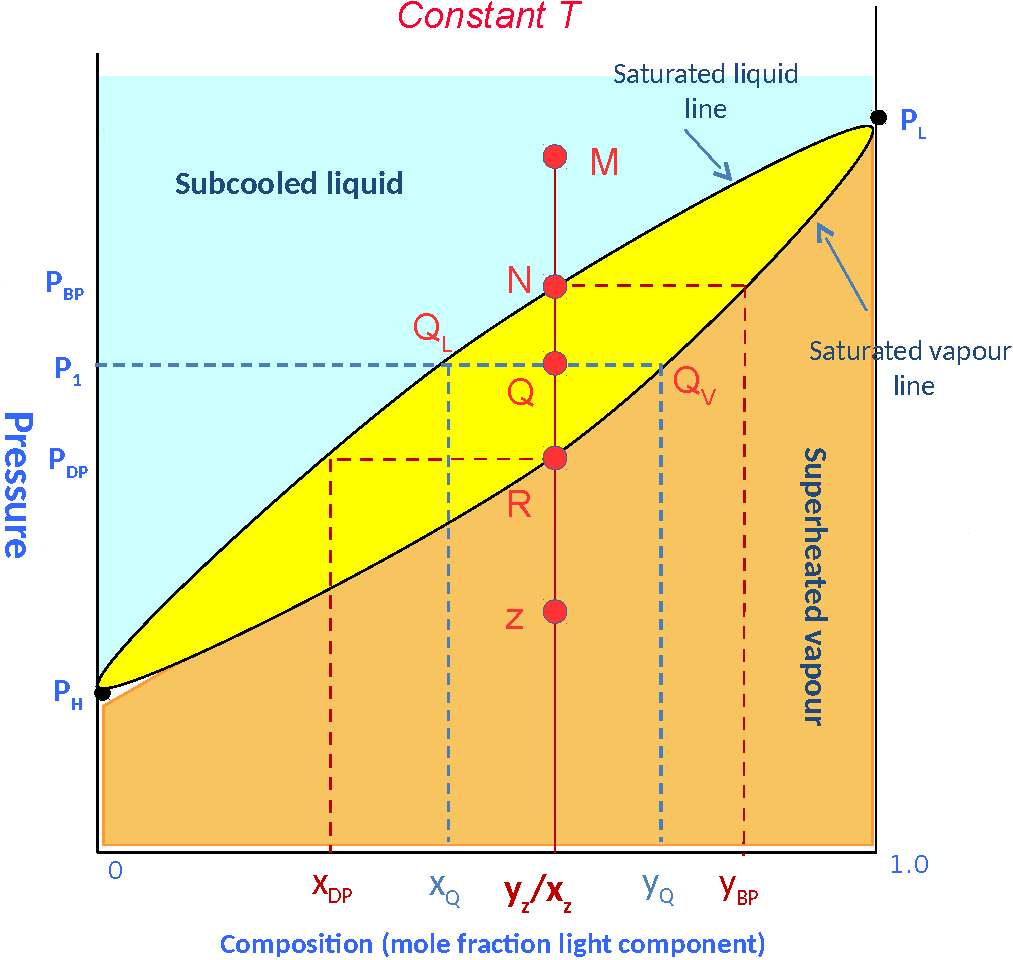
\includegraphics[width=.5\linewidth,clip]{./Pics/VLE_Pxy_Diagram3b}
          \caption{VLE for binary mixture: P-xy diagram at constant temperature.}\label{Figure:Fig1}
        \end{center}
      \end{figure}
      Determine (i)-(ix) from Table~\ref{Table:Tab1},\marks{10}
      \begin{table}[h]
        \begin{center}
          \begin{tabular}{||c| c | c | c | c ||}
            \hline\hline
            {\bf Coordinate} & {\bf Pressure} & {\bf Fluid State} & $\mathbf{x}_{1}$ & $\mathbf{y}_{1}$ \\
            \hline
                 M           &   --           &   subcooled liquid & $x_{1}=x_{z}$    & $y_{1}=0$        \\
                 N           &bubble point $\left(P_{BP}\right)$&--& (i)             & (ii)            \\
                 Q           &  --            &     (iii)          & (iv)             & (v)            \\
                 R           &  (vi)          &     --             & (vii)             & (viii)            \\
                 Z           &  --           &     (ix)            & (x)         &  --            \\                 
            \hline\hline
          \end{tabular}
        \end{center}
        \caption{Properties of $P-xy$ phase diagram}\label{Table:Tab1}
      \end{table}
      \solution{
        \begin{enumerate}[(i)]
           \item $x_{1}=x_{z}$;\solmarks{1/10}
           \item $y_{1}=y_{BP}$;\solmarks{1/10}
           \item vapour-liquid mixture;\solmarks{1/10}
           \item $x_{1}=x_{Q}$;\solmarks{1/10}
           \item $y_{1}=y_{Q}$;\solmarks{1/10}
           \item dew point $\left(P_{DP}\right)$;\solmarks{1/10}
           \item $x_{1}=x_{DP}$;\solmarks{1/10}
           \item $y_{1}=y_{z}$;\solmarks{1/10}
           \item superheated vapour;\solmarks{1/10}
           \item $x_{1}=0$;\solmarks{1/10}
        \end{enumerate}
        }
        
%====================================================
%%% Moran & Shapiro (Example 11.5)      
     \item Using the Redlich-Kwong equation of state, develop algebraic expressions for changes in specific entropy $\left(s_{2}-s_{1}\right)$ and internal energy $\left(u_{2}-u_{1}\right)$ of a gas between two states at the same temperature, \ie $T_{1}=T_{2}$, and pressures $P_{1}$ and $P_{2}$.\marks{10}
%====================
        \solution{The RK EOS is explicit in pressure,
           \begin{displaymath}
             P = \frc{R T}{v-b} - \frc{a}{v\sqrt{T}\left(v+b\right)},
           \end{displaymath}
           and in order to obtain $u_{2}-u_{1}$, $s_{2}-s_{1}$ we should integrate
           \begin{displaymath}
             \begin{cases}
               ds = \frc{C_{v}}{T}dT + \Partial[P]{T}{v}dv & \\
               du = C_{v}dT + \left[T\Partial[P]{T}{v}-P\right]dv & \\
             \end{cases}
           \end{displaymath}
          At the isotherm $T_{1}=T_{2}$,\solmarks{2/10}
           \begin{displaymath}
             \begin{cases}
               s_{2}-s_{1} = \displaystyle\int\limits_{v_{1}}^{v_{2}} \Partial[P]{T}{v}dv, & \\
               u_{2}-u_{1} = \displaystyle\int\limits_{v_{1}}^{v_{2}} \left[T\Partial[P]{T}{v}-P\right]dv. & \\
             \end{cases}
           \end{displaymath}
           The limits for the integrals are the specific volumes $v_{1}$ and $v_{2}$ at the two states under consideration. Using $P_{1}$ and $P_{2}$ and the known temperature, $T_{1}=T_{2}=T$, these specific volumes should be readily obtained from the RK EOS. Before integrating, we need to solve the partial differential $\Partial[P]{T}{v}$ for the RK EOS,
           \begin{displaymath}
             \Partial[P]{T}{v} = \frc{R}{v-b} + \frc{a}{2v\left(v+b\right)T^{3/2}}.
           \end{displaymath}
           Now solving for the change in entropy,\solmarks{3/10}
           \begin{eqnarray}
             s_{2}-s_{1} &=& \displaystyle\int\limits_{v_{1}}^{v_{2}} \left[\frc{R}{v-b} + \frc{a}{2v\left(v+b\right)T^{3/2}}\right]dv \nonumber \\
                        &=& R \ln{\left(\frc{v_{2}-b}{v_{1}-b}\right)} + \frc{a}{2bT^{3/2}}\left[\ln{\frc{v_{2}}{v_{1}}}-\ln{\frc{v_{2}+b}{v_{1}+b}}\right] \nonumber \\
                        &=& R \ln{\left(\frc{v_{2}-b}{v_{1}-b}\right)} + \frc{a}{2bT^{3/2}}\ln{\frc{v_{2}\left(v_{1}+b\right)}{v_{1}\left(v_{2}+b\right)}}.\nonumber
           \end{eqnarray}
           For the change in internal energy, the term in bracket\solmarks{2/10}
           \begin{displaymath}
             \left[T\Partial[P]{T}{v}-P\right] = \frc{3a}{2v\left(v+b\right)T^{1/2}},
           \end{displaymath}
           need to be integrated from $v_{1}$ to $v_{2}$,\solmarks{3/10}
           \begin{eqnarray}
             u_{2}-u_{1} &=& \displaystyle\int\limits_{v_{1}}^{v_{2}} \frc{3a}{2v\left(v+b\right)T^{1/2}}dv \nonumber \\
                        &=& \frc{3a}{2bT^{1/2}}\left[\ln{\frc{v_{2}}{v_{1}}} - \ln{\frc{v_{2}+b}{v_{1}+b}}\right] \nonumber \\
                        &=& \frc{3a}{2bT^{1/2}}\left[\ln{\frc{v_{2}\left(v_{1}+b\right)}{v_{1}\left(v_{2}+b\right)}}\right].\nonumber
           \end{eqnarray}
        }
%====================================================
  \end{enumerate}
\end{question}

\clearpage

%%%
%%% QUESTION 05
%%%
\begin{question}
  
%
\begin{enumerate}[a)]

%%%
%%% Johannes Problem 2 (Tutorial 5)
%%%
\item\label{Tut05P2} A process stream contains light species 1 and heavy species 2. A relatively pure liquid stream containing mostly 2 is obtained through a single-stage liquid/vapour separator. Equilibrium mole fractions are $x_{1}$ = 0.002 and $y_{1}$ = 0.950. Assuming that the modified Raoult's law applies, 
\begin{displaymath}
  y_{i} P = x_{i}\gamma_{i}P_{i}^{\text{sat}},
\end{displaymath} 
determine $T$ and $P$ for the separator. The activity coefficients for the liquid phase are given by,
\begin{displaymath}
\ln\gamma_{1} = 0.93x_{2}^{2} \;\;\;\;\;\text{ and }\;\;\;\;\;\ln\gamma_{2}=0.93x_{1}^{2},
\end{displaymath}
and the saturated vapour pressure is given by,
\begin{displaymath}
\ln P^{\text{sat}} = A - \frc{B}{T}\;\;\;\text{with [P] = bar and [T] = [B] = K},
\end{displaymath} 
with $A_{1}=$ 10.08, $B_{1}=$ 2572.0, $A_{2}=$  11.63 and $B_{2}=$ 6254.0.~\marks{13}

%===================
\solution{Given,
\begin{eqnarray}
&& x_{1} = 0.002 \;\;\Longrightarrow \;\; x_{2} = 0.998 \nonumber \\
&& y_{1} = 0.950 \;\;\Longrightarrow \;\; y_{2} = 0.050 \nonumber
\end{eqnarray}
Calculating the activity coefficient,~\solmarks{2/13},
\begin{eqnarray}
&& \ln{\gamma_{1}} = 0.93 x_{2}^{2} \;\;\Longrightarrow \;\; \gamma_{1} = 2.5251 \nonumber \\
&& \ln{\gamma_{2}} = 0.93 x_{1}^{2} \;\;\Longrightarrow \;\; \gamma_{2} = 1.0000 \nonumber
\end{eqnarray}
The modified Raoult's law,~\solmarks{4/13}
\begin{eqnarray}
&& y_{i}P=x_{i}\gamma_{1}P_{i}^{sat} \;\; \Longrightarrow \;\; P=\frc{x_{i}\gamma_{i}P_{i}^{sat}}{y_{i}} \nonumber \\
&& \frc{P_{1}^{sat}}{P_{2}^{sat}} = \frc{x_{2}\gamma_{2}y_{1}}{x_{1}\gamma_{1}y_{2}} = 3754.7028 = \frc{\exp{\left(A_{1}-\frc{B_{1}}{T}\right)}}{\exp{\left(A_{2}-\frc{B_{2}}{T}\right)}}\nonumber
\end{eqnarray}
Solving this equation results in $T=376.45$ K~\solmarks{3/13}. The pressure can now be obtained,~\solmarks{4/13}
\begin{displaymath}
  P=\frc{x_{i}\gamma_{1}P_{1}^{sat}}{y_{1}} = 0.1368\text{ bar}
\end{displaymath}
}
%==================

% Nguyen (page 106, Ex 5.1-1)
\item Determine the temperature and composition of the first bubble created from a saturated liquid mixture of benzene and toluene containing 45 mol$\%$ percent of benzene at 200 kPa. Benzene and toluene mixtures may be considered as ideal. Given,~\marks{7}
\begin{displaymath}
\ln{P^{sat}} = A - \frc{B}{T+C}\;\;\text{ with [P] = kPa and  [T] = [B] = [C] = K},
\end{displaymath}
and
\begin{center}
\begin{tabular}{ c  c  c  c }
\hline
           & ${\bf A}$  &  ${\bf B}$  & ${\bf C}$ \\
\hline
Benzene    & 14.1603    &  2948.78    & -44.5633 \\
Toluene    & 14.2514    &  3242.38    & -47.1806 \\
\hline
\end{tabular}
\end{center}

%=================
\solution{From Raoult's law, 
\begin{displaymath}
y_{i} = \frc{x_{i}P_{i}^{sat}}{P}
\end{displaymath}
with benzene (1) and toluene (2),~\solmarks{1/7}
\begin{displaymath}
P = x_{1}P_{1}^{sat} + x_{2}P_{2}^{sat}
\end{displaymath}
leading to the bubble point temperature of the mixture benzene-toluene~\solmarks{3/7}
\begin{displaymath}
P = x_{1}\exp{\left(A_{1}-\frc{B_{1}}{T+C_{1}}\right)} + x_{2}\exp{\left(A_{2}-\frc{B_{2}}{T+C_{2}}\right)} \;\Longrightarrow\; T= 391.73\text{ K}
\end{displaymath}
Calculating the saturation pressure and mole fraction of benzene in the vapour phase,~\solmarks{3/7}
\begin{eqnarray}
&& P_{1}^{sat} = \exp{\left(A_{1}-\frc{B_{1}}{T - C_{1}}\right)} = 289.01\text{ kPa} \nonumber \\
&& y_{1} = \frc{x_{1}P_{1}^{sat}}{P} = 0.6503 \;\text { and } y_{2}=1-y_{1} = 0.3497 \nonumber
\end{eqnarray}
}
%=================

\end{enumerate}
\end{question}


\vfill
\paperend
 


\vfill 



%\begin{comment}
{
  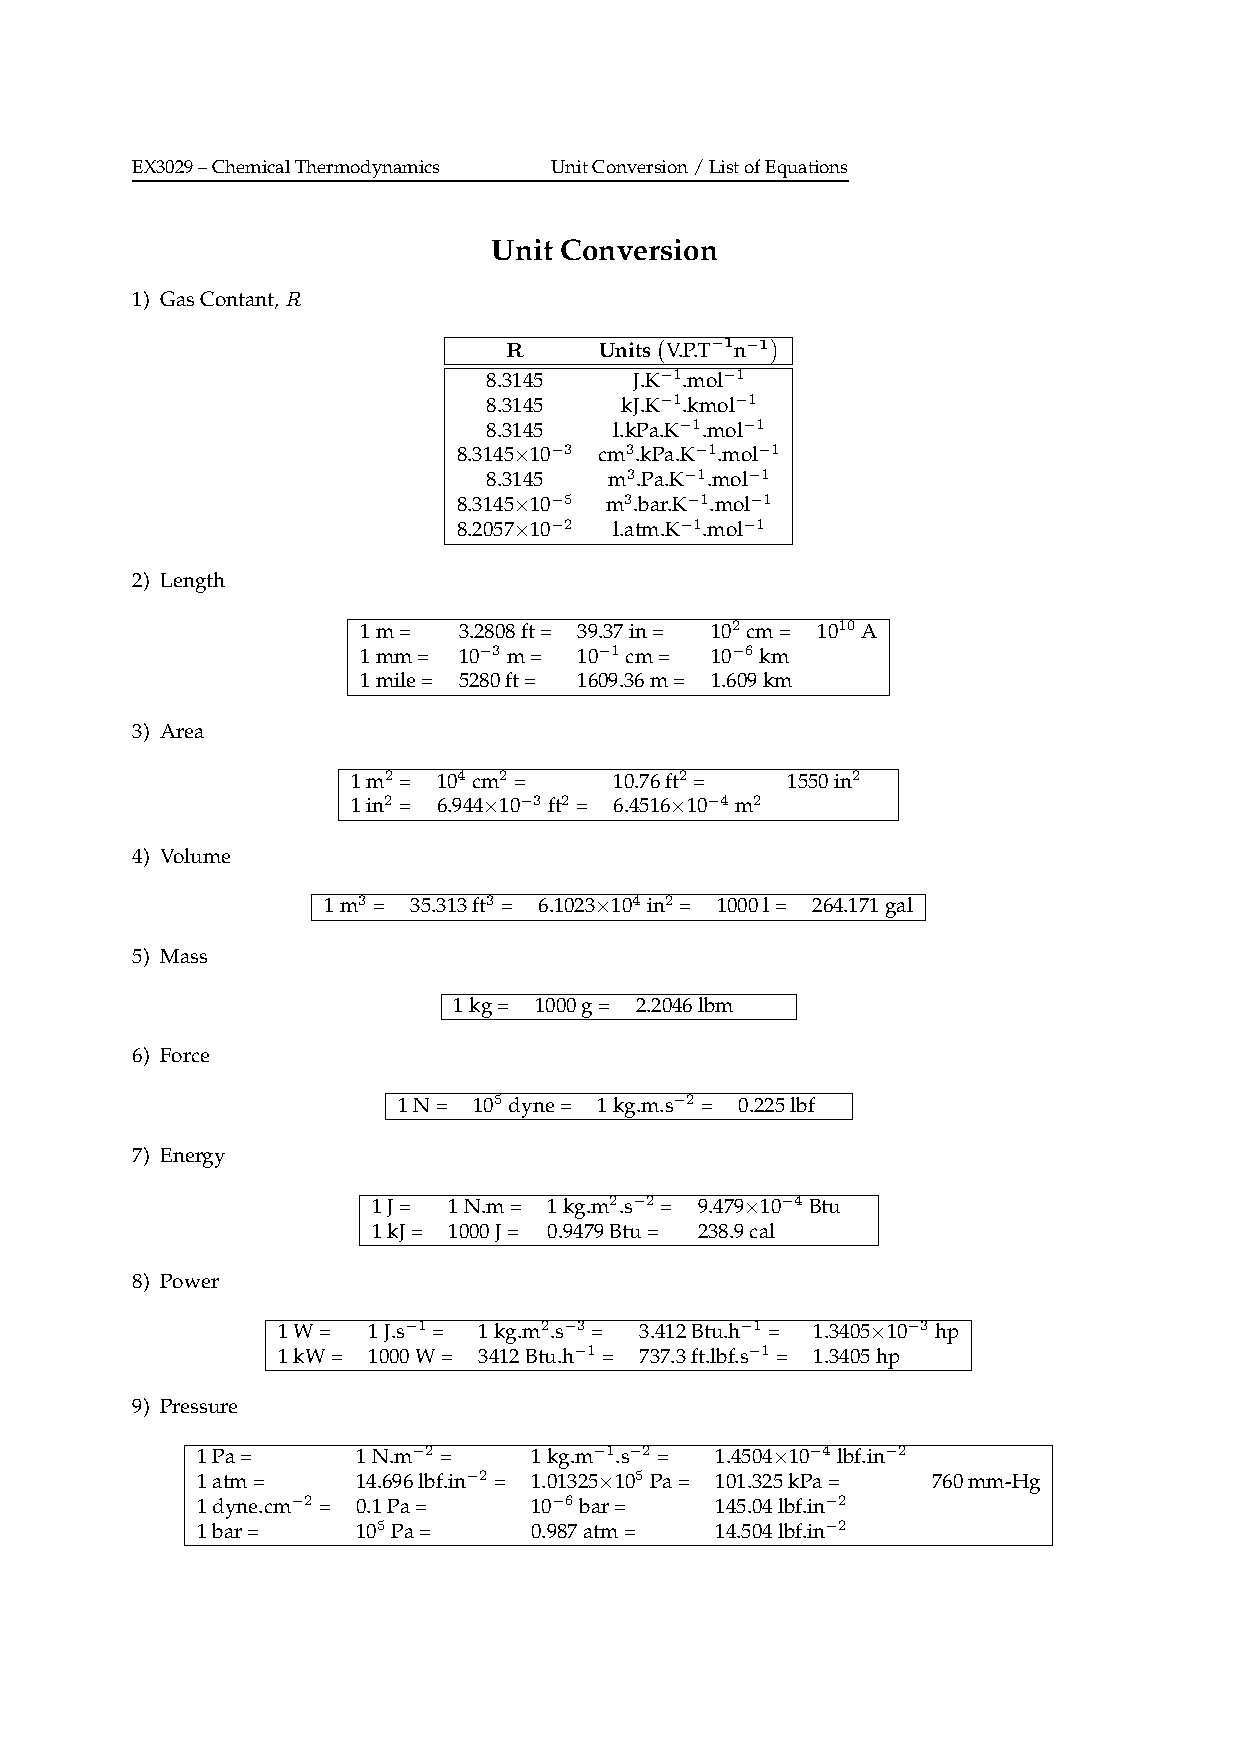
\includepdf[pages=-,fitpaper]{./Pics/EquationsList}
}
%\end{comment}



\end{document}
